\documentclass{standalone}
\usepackage{tikz}
\usetikzlibrary{positioning}

\begin{document}

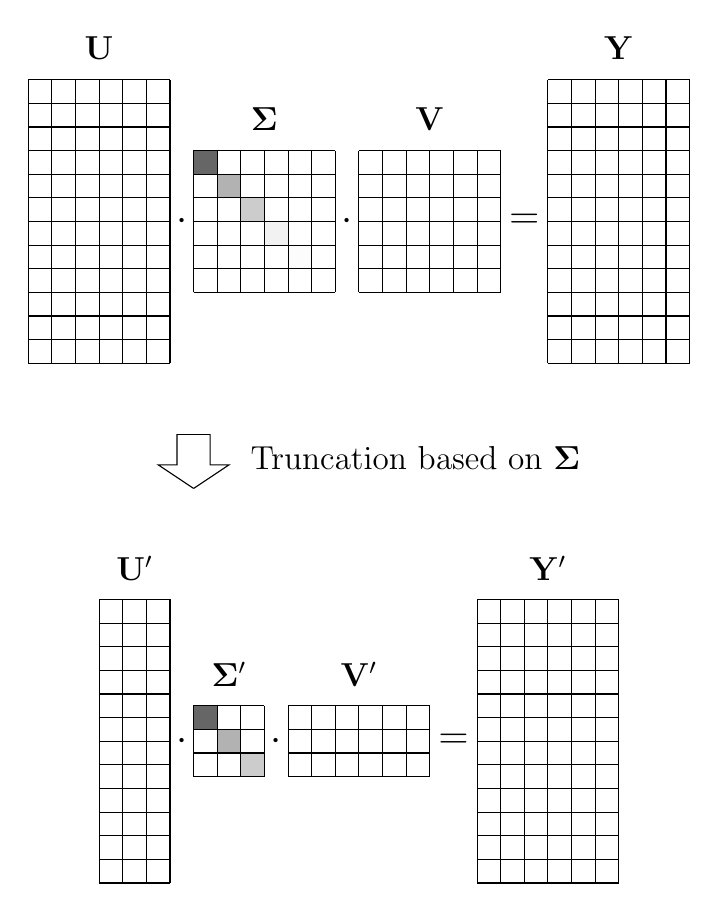
\begin{tikzpicture}[scale=.3]
\begin{scope}[yshift=0]

    \draw[step=1, black, shift={(0, 0)}] (0,0) grid (6,12);
    \draw[step=1, black, shift={(7, 3)}] (0,0) grid (6,6);
    \draw[step=1, black, shift={(14, 3)}] (0,0) grid (6,6);
    \draw[step=1, black, shift={(22, 0)}] (0,0) grid (6,12);

    \node[yshift=1mm] at (3, 13) {\large $\mathbf{U}$};
    \node[yshift=1mm] at (10, 10) {\large $\mathbf{\Sigma}$};
    \node[yshift=1mm] at (17, 10) {\large $\mathbf{V}$};
    \node[yshift=1mm] at (25, 13) {\large $\mathbf{Y}$};

    \node at (6.5, 6) {\Large $\cdot$};
    \node at (13.5, 6) {\Large $\cdot$};
    \node at (21, 6) {\Large $=$};

    \begin{scope}[shift={(7,9)}]
    \draw[fill=black!60!white, shift={(0, 0)}] (0, 0) rectangle (1, -1);
    \draw[fill=black!30!white, shift={(1,-1)}] (0, 0) rectangle (1, -1);
    \draw[fill=black!20!white, shift={(2,-2)}] (0, 0) rectangle (1, -1);
    \draw[fill=black!5!white,  shift={(3,-3)}] (0, 0) rectangle (1, -1);
    \draw[fill=black!1!white,  shift={(4,-4)}] (0, 0) rectangle (1, -1);
    \end{scope}

    % \node[anchor=center] at (14, -2) {SVD of the farfield matrix};

\end{scope}

\begin{scope}[xshift=7cm, yshift=-4cm]

    \draw (-.7, 1) -- ++(0, -1.3) -- ++(-.8, 0) -- ++(+1.5, -1);
    \draw (+.7, 1) -- ++(0, -1.3) -- ++(+.8, 0) -- ++(-1.5, -1);
    \draw (-.7, 1) -- (+.7, 1);

    \node[anchor=west] at (2, 0) {\large Truncation based on $\mathbf{\Sigma}$};
    
\end{scope}

\begin{scope}[xshift=3cm, yshift=-22cm]

    \draw[step=1, black, shift={(0, 0)}] (0,0) grid (3,12);
    \draw[step=1, black, shift={(4, 4.5)}] (0,0) grid (3,3);
    \draw[step=1, black, shift={(8, 4.5)}] (0,0) grid (6,3);
    \draw[step=1, black, shift={(16, 0)}] (0,0) grid (6,12);

    \node[yshift=1mm] at (1.5, 13) {\large $\mathbf{U'}$};
    \node[yshift=1mm] at (5.5, 8.5) {\large $\mathbf{\Sigma'}$};
    \node[yshift=1mm] at (11, 8.5) {\large $\mathbf{V'}$};
    \node[yshift=1mm] at (19, 13) {\large $\mathbf{Y'}$};

    \node at (3.5, 6) {\Large $\cdot$};
    \node at (7.5, 6) {\Large $\cdot$};
    \node at (15, 6) {\Large $=$};


    \begin{scope}[shift={(4,7.5)}]
        \draw[fill=black!60!white, shift={(0, 0)}] (0, 0) rectangle (1, -1);
        \draw[fill=black!30!white, shift={(1,-1)}] (0, 0) rectangle (1, -1);
        \draw[fill=black!20!white, shift={(2,-2)}] (0, 0) rectangle (1, -1);
    \end{scope}

    % \node[anchor=center] at (11, -2) {Truncated SVD};

\end{scope}
\end{tikzpicture}

\end{document}
